\documentclass{standalone}
\usepackage{tikz}
\usepackage{amsmath}
\usetikzlibrary{matrix}
\begin{document}

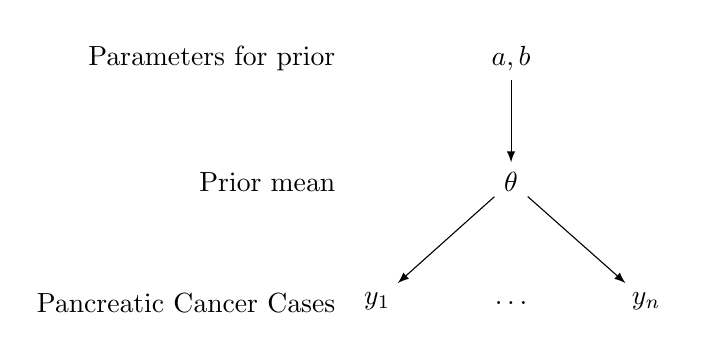
\begin{tikzpicture}
\matrix[matrix of math nodes, column sep=30 pt, row sep=30 pt] (mat)
{
    & a, b & \\ 
    & \theta &\\
    y_1 & \ldots & y_n \\
};

\draw[->,>=latex] (mat-1-2) -- (mat-2-2);
\draw[->,>=latex] (mat-2-2) -- (mat-3-1);
\draw[->,>=latex] (mat-2-2) -- (mat-3-3);

\node[anchor=east] at ([xshift =-60pt]mat-1-2) 
{Parameters for prior};
\node[anchor=east] at ([xshift =-60pt]mat-2-2) 
{Prior mean};
\node[anchor=east] at ([xshift =-60pt]mat-3-2) 
{Pancreatic Cancer Cases};

\end{tikzpicture}
\end{document}
